\documentclass[12pt]{article}

\pagestyle{empty}
\setcounter{secnumdepth}{2}

\topmargin=0cm
\oddsidemargin=0cm
\textheight=22.0cm
\textwidth=16cm
\parindent=0cm
\parskip=0.15cm
\topskip=0truecm
\raggedbottom
\abovedisplayskip=3mm
\belowdisplayskip=3mm
\abovedisplayshortskip=0mm
\belowdisplayshortskip=2mm
\normalbaselineskip=12pt
\normalbaselines

\usepackage{graphicx}
\usepackage{float}
\usepackage{titlesec}

\setcounter{secnumdepth}{3}

\begin{document}

\vspace*{0.5in}
\centerline{\bf\Large Design Document}

\vspace*{0.5in}
\centerline{\bf\Large Team PB-PI}

\vspace*{0.5in}
\centerline{\bf\Large March 18, 2018}

\vspace*{1.5in}
\begin{table}[htbp]
\caption{Team}
\begin{center}
\begin{tabular}{|r | c|}
\hline
Name & ID Number \\
\hline\hline
Alissa Bellerose & 27377320 \\
Sabrina D'Mello & 27739486 \\
Melanie Damilig & 40032420 \\
Tobi Decary-Larocque & 27407645 \\
Zain Farookhi & 26390684 \\
Giulia Gaudio & 27191766 \\
Jason Kalec & 40009464 \\
Damian Kazior & 40016168 \\
Johnny Mak & 40002140 \\
Philip Michael & 40004861 \\
Ramez Nicolas Nahas & 26718108 \\
Steven Tucci & 40006014 \\
Shunyu Wang & 40043915 \\
\hline
\end{tabular}
\end{center}
\end{table}

\clearpage

\section{Introduction}
The primary goal of this project is to create an application which allows students to keep track of their money. The MyMoney application allows students to create an account which provides them with different options to keep track of their money and spending habits through the graphical user interface. The application allows the user to create a transaction, either deposit or withdraw. It will also allow the user an option to display balance, show transaction history and clear history. 


\subsection{Purpose}
The purpose of this document is to provide details on the architectural design, software design and internal design of the MyMoney application. The software architecture that was chosen for the application will be described in high level detail and a class diagram will be depicted. The software interface will have screenshots of the graphical user interface and a high level description of how the user will interacts with the system.


\subsection{Scope}
This document is intended to provide a basis for implementation. The architecture and software processes will be explained in great detail in order to facilitate implementation and be an effective reference tool. 


\subsection{Definitions and Abbreviations}

\subsubsection{Definitions}
\begin{table}[H]
\caption{Definitions}
\begin{center}
\begin{tabular}{|p{3cm}|p{12cm}|}
\hline
Term & Definition \\
\hline\hline
Model View Controller & The architecture used in the MyMoney application. It consists of 3 individual components the model, the view and the controller.  \\
\hline

\end{tabular}
\end{center}
\end{table}

\subsubsection{Abbreviations}

\begin{table}[H]
\caption{Abbreviations}
\begin{center}
\begin{tabular}{|p{3cm}|p{12cm}|}
\hline
Abbreviation & Term \\
\hline\hline
GUI & Graphical User Interface  \\
\hline
MVC & Model View Controller \\
\hline
UML & Unified Modeling Language \\
\hline
ORM & Object Relational Mapping \\
\hline
API & Application Programming Interface \\
\hline
CRUD & Create, Read, Update, Delete \\
\hline
SQL & Structured Query Language \\
\hline

\end{tabular}
\end{center}
\end{table}


\subsection{References}

Pressman, Roger S. Software Engineering: A Practitioner's Approach. 5th ed. Toronto: McGraw-Hill, 2001. 

Larman, Craig. Applying UML and patterns: an introduction to object-Oriented analysis and design and the unified process. Prentice-Hall, 2005.


\subsection{Overview}
This document is divided into three major parts; the architectural design, the detailed design and the dynamic design scenarios. The architectural and software design will be described in detail in their respective individual parts.


\section{Architectural Design}

\subsection{Architectural Diagram}
The MyMoneyApp uses a simple MVC architecture with an observer pattern to notify of data changes across the view and model. The MVC pattern is known as the Model - View - Controller pattern.  Along with the MVC architecture the application also has singleton patterns. The singleton design pattern is used for only instantiating one object from a class. The singleton pattern was used for the creating the default GUI layout for the user and the initial connection to the applications database. The most prominent architecture design used for creating the MyMoneyApp is the MVC pattern.

\begin{figure}[h!]
  \centering
  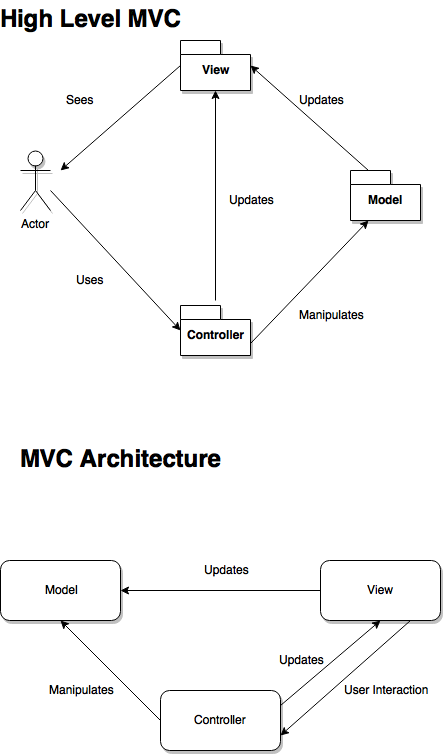
\includegraphics[width=110mm]{MVC.png}
  \caption{MVC Diagrams}
\end{figure}

% Doenst support static gif. we'll need to convert to another format
%\begin{figure}[h!]
%  \centering
%  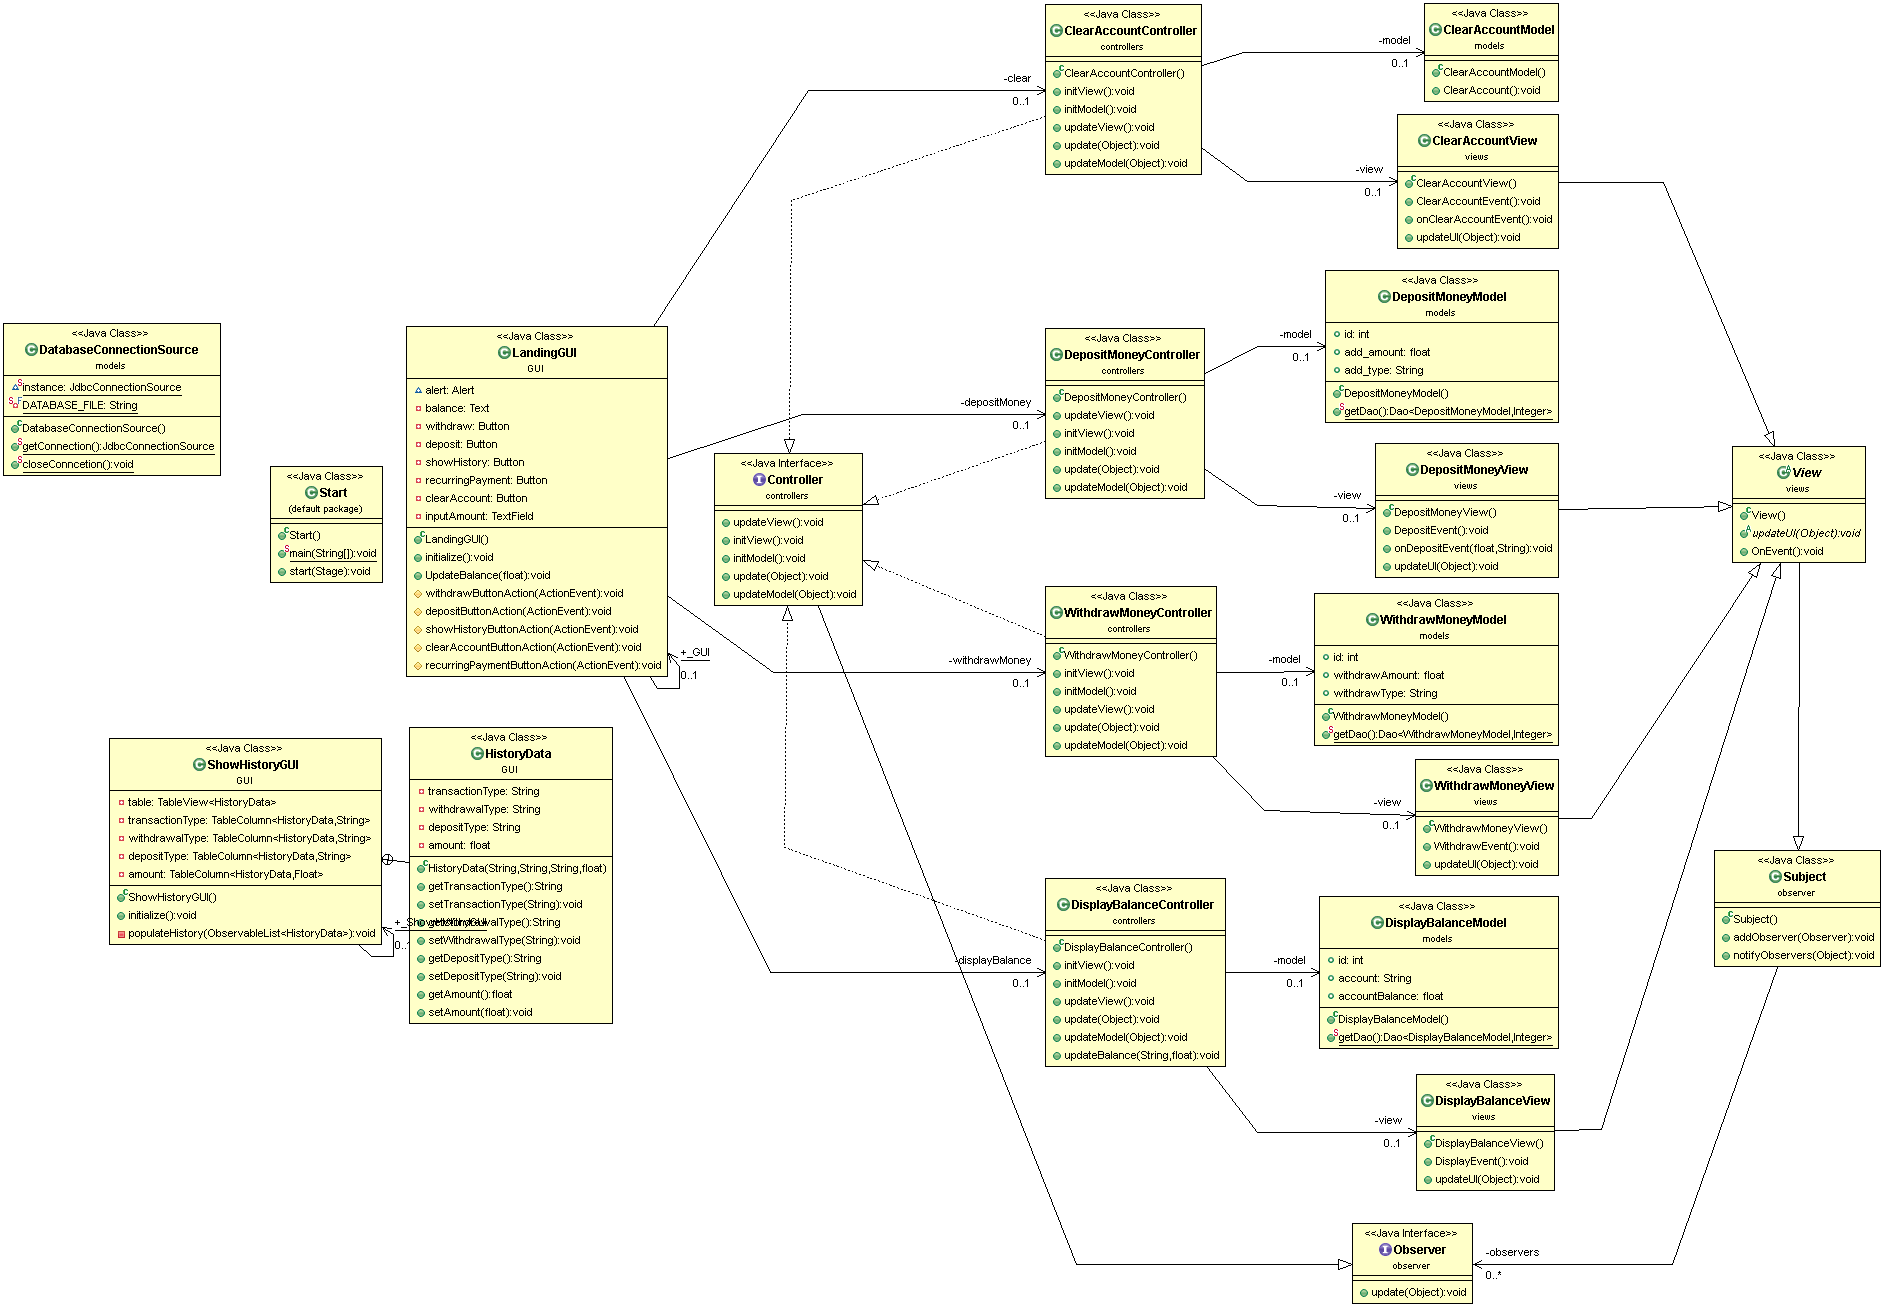
\includegraphics[width=110mm]{class_diagram.gif}
%  \caption{MVC Diagrams}
%\end{figure}



\subsubsection{Model}
The model component is where we store our business models and data. For that, we use an abstraction known as ORM (Object Relational Mapping). The ORM allows us to perform CRUD operations on our data without writing hardcoded specific database queries. This allows us to perform queries on a higher abstraction level and be able to switch our data store without ever rewriting new query code. 


\subsubsection{View}
The view component layer is where the user interacts with the system. In our case this is the GUI, but the view layer does not necessarily have to be a GUI. The view displays our models, collection of models, or any mix of model data. This means that our views does not necessarily have to be binded to one model. Since the user interacts with the view, all view logic is done on the view layer. As a result, when a user presses a button, the view captures the event, then it creates a message and passes this to the controller to handle the event. Since we are using the Observer pattern, the view is a Subject. That means the view/subject will notify its observer with the data. Therefore, there is no direct connection with the controller. 


\subsubsection{Controller}
The controller component is an intermediary between the view and model. The controller is the observer. It subscribes to the view events, and handles any messages passed to it from the view.  This means that the user interacts with the view, and not the controller. However, the view delegates view interaction to the controller. When an event happens in the view, the view passes the message to the controller. The controller receives the message and decides what to do with the message. The controller reads the message with the view data, and reflects the view changes across the model. The controller directly manipulates the model data, and persists the new model data to the model layer where it gets automatically updated into our database. Once the model gets updated, the controller takes any model changes and sends a message back to the view with the new updated view data. The view then takes this message and reflects the view/gui changes with the data.



\subsubsection{View/Controller Interface}

The view and controllers interface each other by using the Observer pattern. The view is the subject, and the controller is the observer. The controller subscribes to the subject’s event.
When there is a view event, the view notifies the observer of an event, and the controller handles it, and submits back a response after it has processed the event.

\subsubsection{Controller/Model Interface}

The controller does not directly manipulate the model through database queries, but instead it manipulates the model’s high level ORM API.

\subsection{Rationale}
The reason why the MyMoneyApp uses the MVC model with the observer pattern, is that it allows us to independently manage business logic from the view logic. We could create new views without ever worrying about how the controller and model work. This allows for new controllers and models to be created, tested, debugged, and integrated in parallel. With this architecture, we have an extremely flexible system that allows us to have different views without ever worrying about how the model or controller even work. Whether the views are a GUI, or command line, the model does not care. In fact, our model does not even know a view exists. In a lot of MVC patterns, there is some connection between the model and view. We decided to not use this approach. Our architecture is all about message passing. There are no direct connections between the view and controller, and no direct connection between the view and model. We pass messages between the view and controller through the observer pattern. This allows us to swap views without the controller ever knowing. Our controllers are responsible for notifying the model of the changes, and notifying the view of the model changes.

There are different variations on the MVC pattern. We use a pull model approach. This means, that if the model changes, the view does not get updated right away. The view must pull or refresh the data from the model. As a result, if our view data changes, then the model is automatically updated. There is a one way binding between our view and model.

We chose the one where we treat the model as a simple value object. There is a very good reason why this is done. The team discussed about this topic, from the experience of the group when you put all the logic in the models, you get very bloated models that are not very interchangeable across different views. Our way gives us a very clean and extensible way of interchanging our model across different domains. 



\subsection{Subsystem Interface Specifications}
All the subsystems interact with a message passing interface. Each view has a custom data type message that is passes to the other subsystems. The corresponding controller should expect the custom message and handle it appropriately. When messages are passed around, they are passed as high level Object class types, the views and controllers must down cast the object to its expected message type/class.

\subsubsection{View Interface Subsystem}

\begin{table}[H]
  \caption{updateUi method spec}
  \begin{center}
    \begin{tabular}{|l|p{10cm}|}

      \hline
      \bf Method: & void updateUI(Object data)\\
		\hline
      \bf Purpose: & To notify the view that it should update its view state with the current data message.
This is the controller to view interface. This is used when the controller sends a message to the view.
)\\
\hline
      \bf Parameters: & Object data. The data/message that the current view should unpack/cast and update its state with.The view should cast the object to its own object type.\\
		\hline
      \bf Valid data: &  An object of type that is known to the view and controller\\
      \hline
      \bf Invalid data: &  Null, or an unknown data message type. The view should handle invalid data in an expected manner, and should not throw any exceptions up the system interface.\\
      \hline

    \end{tabular}
  \end{center}
\end{table}

\begin{table}[H]
  \caption{notifyObservers method spec}
  \begin{center}
    \begin{tabular}{|l|p{10cm}|}
      \hline
      \bf Method: & void notifyObservers(Object data)\\
		\hline
      \bf Purpose: &  Notify all dependent observers/controllers with a new message/data. This is the view to controller interface. This is used when the view wants to send a message to the controller.\\
		\hline
      \bf Parameters: & Object data. The data/message that the current view sends to its controller when the view wants to notify the controller of a view event or change.\\
		\hline
      \bf Valid data: &  An object of type that is known to the view and controller\\
      \hline
      \bf Invalid data: & Null, or an unknown data message type. The view should handle invalid data in an expected manner, and should not throw any exceptions up the system interface.\\
      \hline

    \end{tabular}
  \end{center}
\end{table}

\begin{table}[H]
  \caption{addObserver method spec}
  \begin{center}
    \begin{tabular}{|l|p{10cm}|}
      \hline
      \bf Method: & void addObserver(Observer observer)\\
		\hline
      \bf Purpose: & Add an observer/controller to the current subject/view.\\
		\hline
      \bf Parameters: & Observer observer. The controller that subscribes to the view/subject’s events or changes.\\
		\hline
      \bf Valid data: & An observer object that should be expected to handle the view’s messages.\\
      \hline
      \bf Invalid data: &Null, or an unknown controller type that would not know how to handle the view’s messages.\\
      \hline

    \end{tabular}
  \end{center}
\end{table}

\subsubsection{Controller Interface Subsystem}

\begin{table}[H]
  \caption{initModel method spec}
  \begin{center}
    \begin{tabular}{|l|p{10cm}|}
      \hline
      \bf Method: & void initModel()\\
		\hline
      \bf Purpose: & Initialize any model or models that the controller needs to update or create.\\
		\hline
      \bf Parameters: & None.\\
		\hline
    \end{tabular}
  \end{center}
\end{table}

\begin{table}[H]
  \caption{initView method spec}
  \begin{center}
    \begin{tabular}{|l|p{10cm}|}
      \hline
      \bf Method: & void initView()\\
		\hline
      \bf Purpose: &  Initialize the view and setup any needed view logic.\\
		\hline
      \bf Parameters: & None.\\
		\hline
    \end{tabular}
  \end{center}
\end{table}

\begin{table}[H]
  \caption{updateView method spec}
  \begin{center}
    \begin{tabular}{|l|p{10cm}|}
      \hline
      \bf Method: & void updateView()\\
		\hline
      \bf Purpose: & Tells the controller's attached view to update its ui. This method is called after any model changes have happened, and the view needs to reflect these changes.\\
		\hline
      \bf Parameters: & None.\\
		\hline
    \end{tabular}
  \end{center}
\end{table}

\begin{table}[H]
  \caption{update method spec}
  \begin{center}
    \begin{tabular}{|l|p{10cm}|}
      \hline
      \bf Method: & void update(Object data)\\
		\hline
      \bf Purpose: & Update the controller/observer data/state. Update the model with the new changes from the view’s data/message.\\
		\hline
      \bf Parameters: & Object - data, this is the corresponding data message passed from the view's notifyObserver(Object data) call the object is usually going to be type casted to the specified data type depending on the what the view's data is. the data reflects the state of the view\\
		\hline
      \bf Valid data: & An object of type that is known to the view and controller\\
      \hline
      \bf Invalid data: &  Null, or an unknown data message type. The controller should handle invalid data in an expected manner, and should not throw any exceptions up the system interface.\\
      \hline

    \end{tabular}
  \end{center}
\end{table}


\subsubsection{Model Interface Subsystem}
For our model, we are using an ORM called ORMLite. It allows us persist our business objects to a database using a high level api and avoid us having to write our own custom and insecure SQL queries. 

\subsection{System Topology}
The MyMoneyApp is to be used by a single user and ran on a single computer. There will be no need for networked communications or internet connections for the app to work. This allows us to easy distribute the app and integrate all the components into a single executable.


\section{Detailed Design}
The primary User Interface used in the system design, was created using Java FX, which is quite similar to Java Swing. This GUI gives users the ability to interact with the core necessary aspects of the system in order to obtain a satisfactory user experience.

User interactions:\\
User can enter an amount and then press “withdraw amount” to deduct from the current balance\\
User can enter an amount and then press “deposit amount” to increase the current balance\\
User can press edit transaction to change various elements of the current transaction\\
The user can delete their current account\\
The user can press “Set Up recurring payment” to have money deducted at specified intervals or at specific times.\\


\subsection{View Subsystem}
The view subsystem interface connecting model and view is utilized whenever the model is changed in some way and thus the view must be updated to reflect and display the new model.

\subsection{Model Subsystem}
The model subsystem interface connecting controller and model is utilized whenever a user wishes to give input which would result in a change to the data stored in model. The controller thus makes use of this interface to update the model.

\subsection{Controller Subsystem}
The controller subsystem interface connecting the view and controller is utilized whenever the controller needs to render data from the view and when the controller must send data to the view such as updated data or to display an error message.

The systems main interface is composed of various elements required to manage ones money.
There are basic options such as “Withdraw Amount”, “Deposit Amount” and “Show Balance”. There are also advanced options such as “Clear History”, “Show History” and “Show GUI”. The User interface has a “Enter amount…” box where one can enter the amount of money they may wish to deposit or withdraw. The app is constantly displaying the users Current Balance so they will constantly be aware of how much money they currently have.\\

% Screenshot of the app window
%\begin{figure}[h!]
%  \centering
%  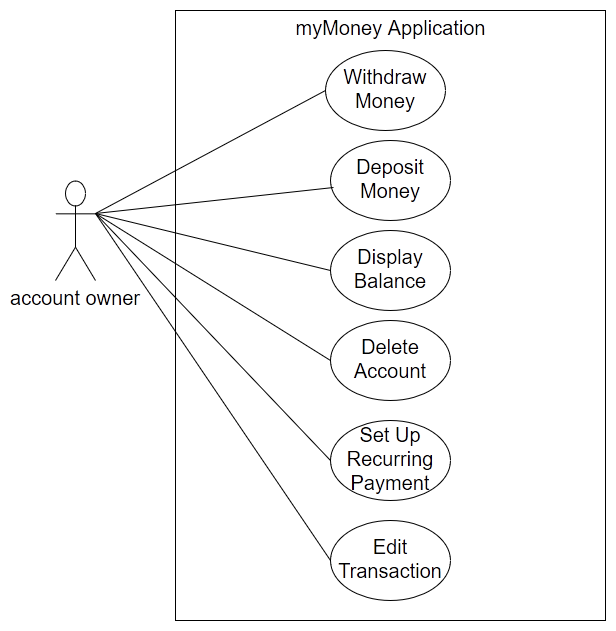
\includegraphics[width=110mm,natwidth=616,natheight=631]{Use_Case_Diagram.png}
%  \caption{MyMoney Application Window}
%\end{figure}

\textbf{Methods}\\
\vspace*{-0.2in}
\begin{enumerate}
  \item initialize(): Gets connection to database, create GUI object referencing the GUI on screen to be used in the view. Initializes necessary controllers, once done close connection to database.
  \item UpdateBalace(balance): When a change is made the balance on screen is updated to reflect the current balance.
\end{enumerate}

\subsubsection{Basic Options}
The basic options subsection of the GUI is displayed as such all functionality that the user will be using frequently such as deposit, withdraw and show history will be available here.

% Basic Options Image
%\begin{figure}[h!]
%  \centering
%  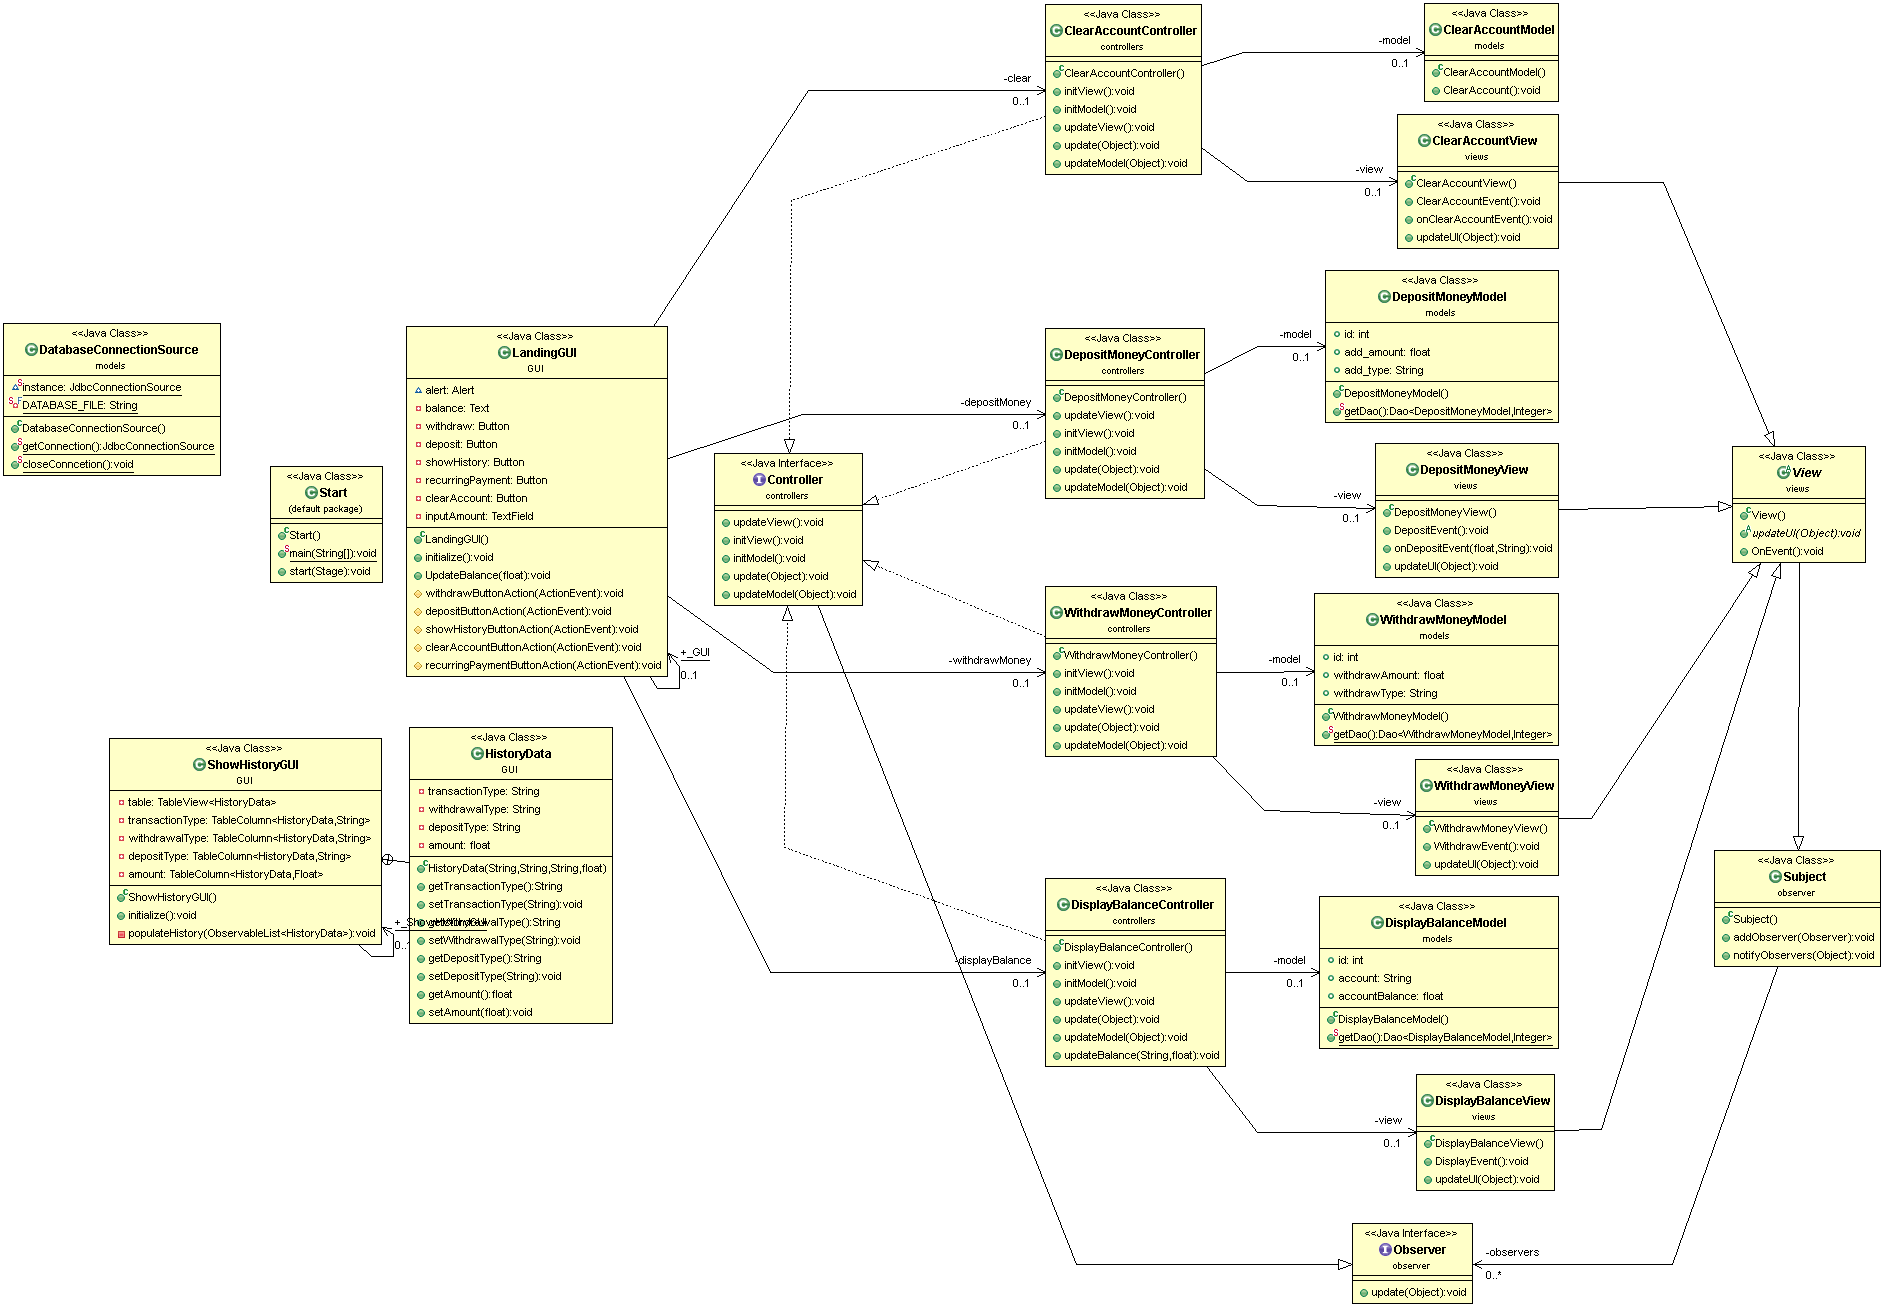
\includegraphics[width=110mm]{class_diagram.gif}
%  \caption{Basic Options}
%\end{figure}

\subsubsection{Advanced Options}
The advanced options subsection of the GUI is displayed as such all functionality that is not frequented often such as setup recurring payment and clear account will be available here.

% Advanced Options Image
%\begin{figure}[h!]
%  \centering
%  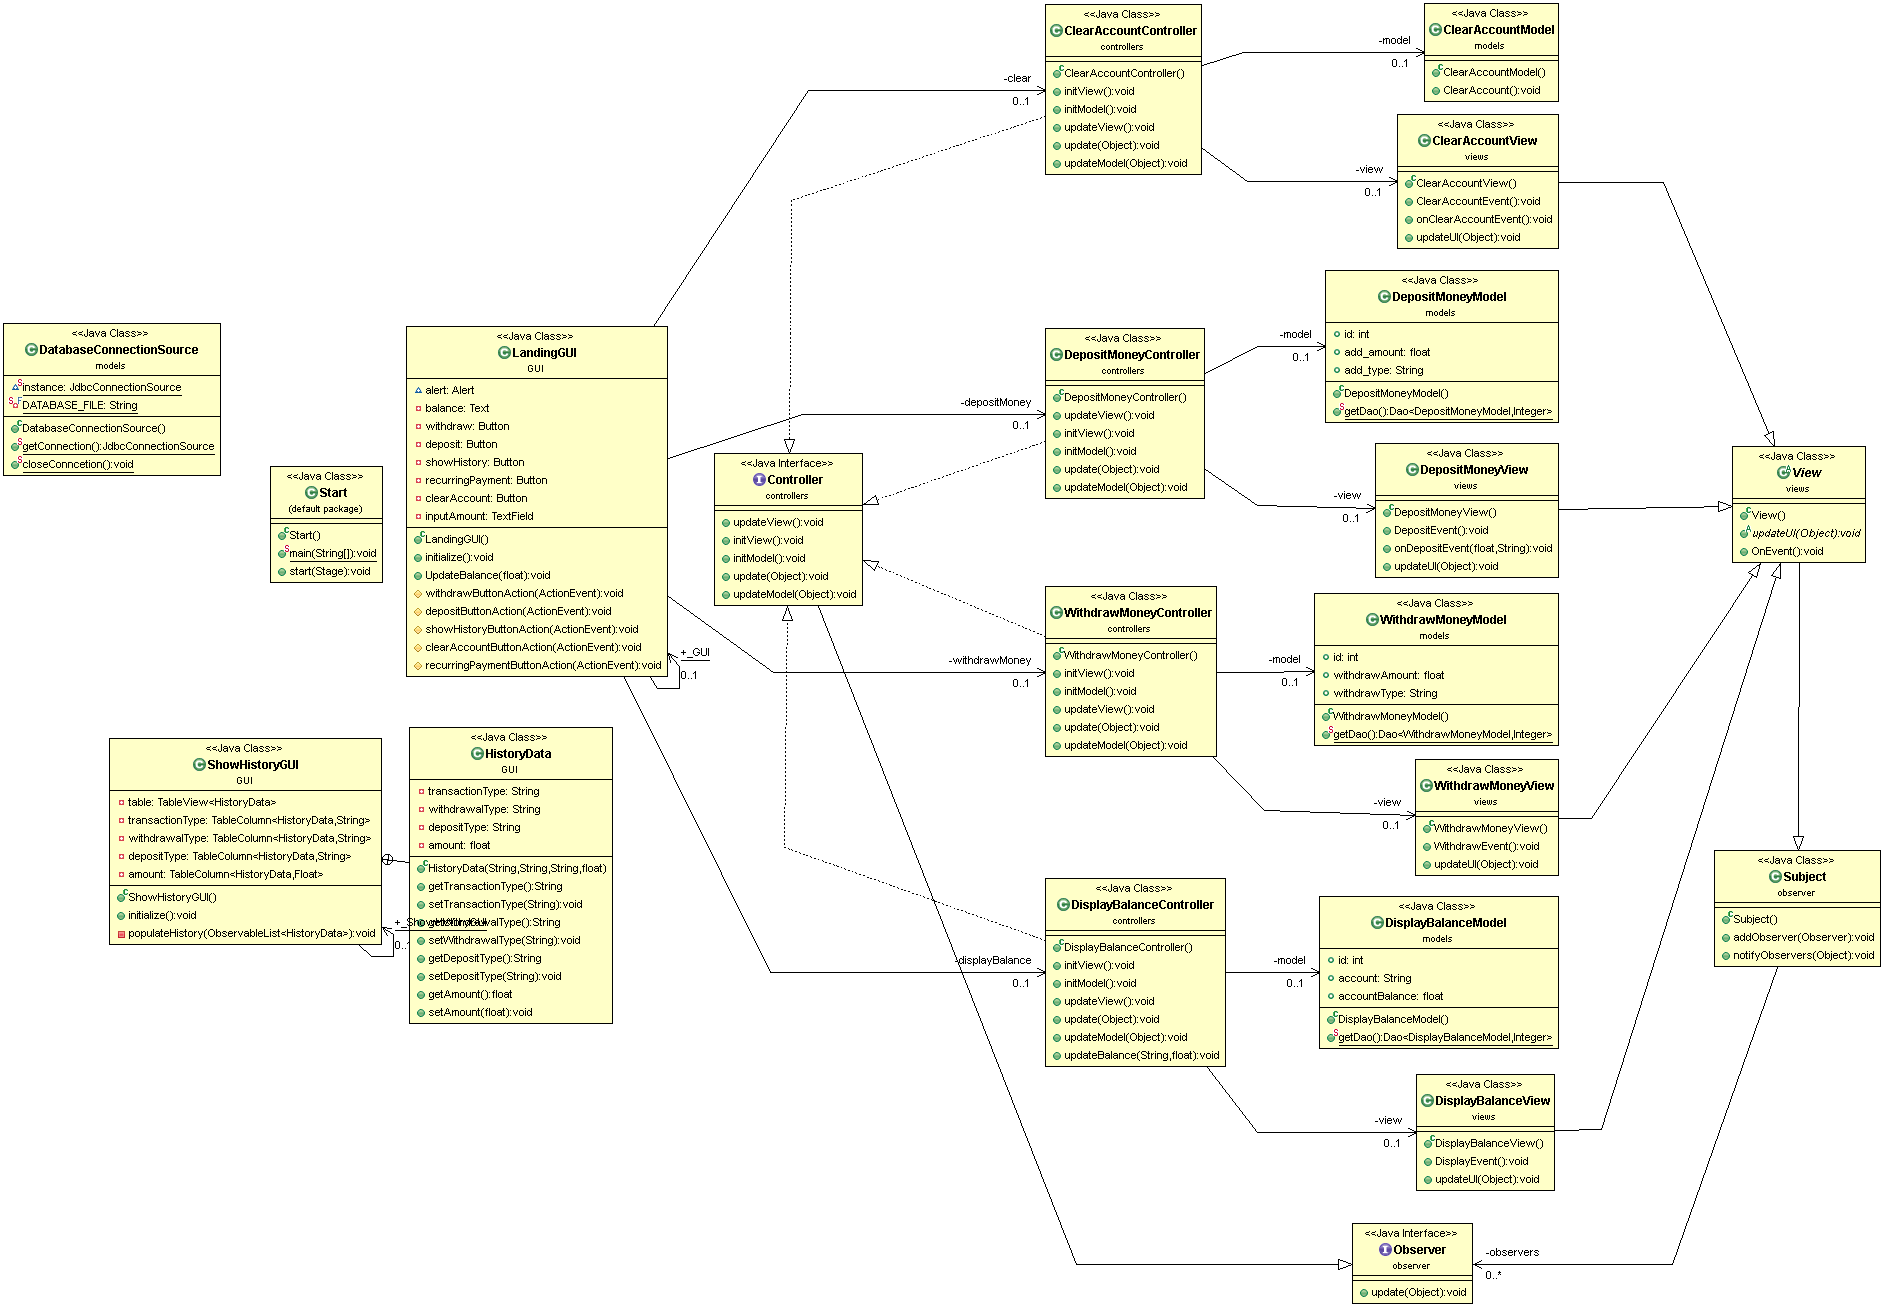
\includegraphics[width=110mm]{class_diagram.gif}
%  \caption{Advanced Options}
%\end{figure}

\subsubsection{Withdraw Button}
The withdraw button of the basic options subsection when clicked on will deduct the specified number in “Enter Amount” from the current balance

% Withdraw button Image
%\begin{figure}[h!]
%  \centering
%  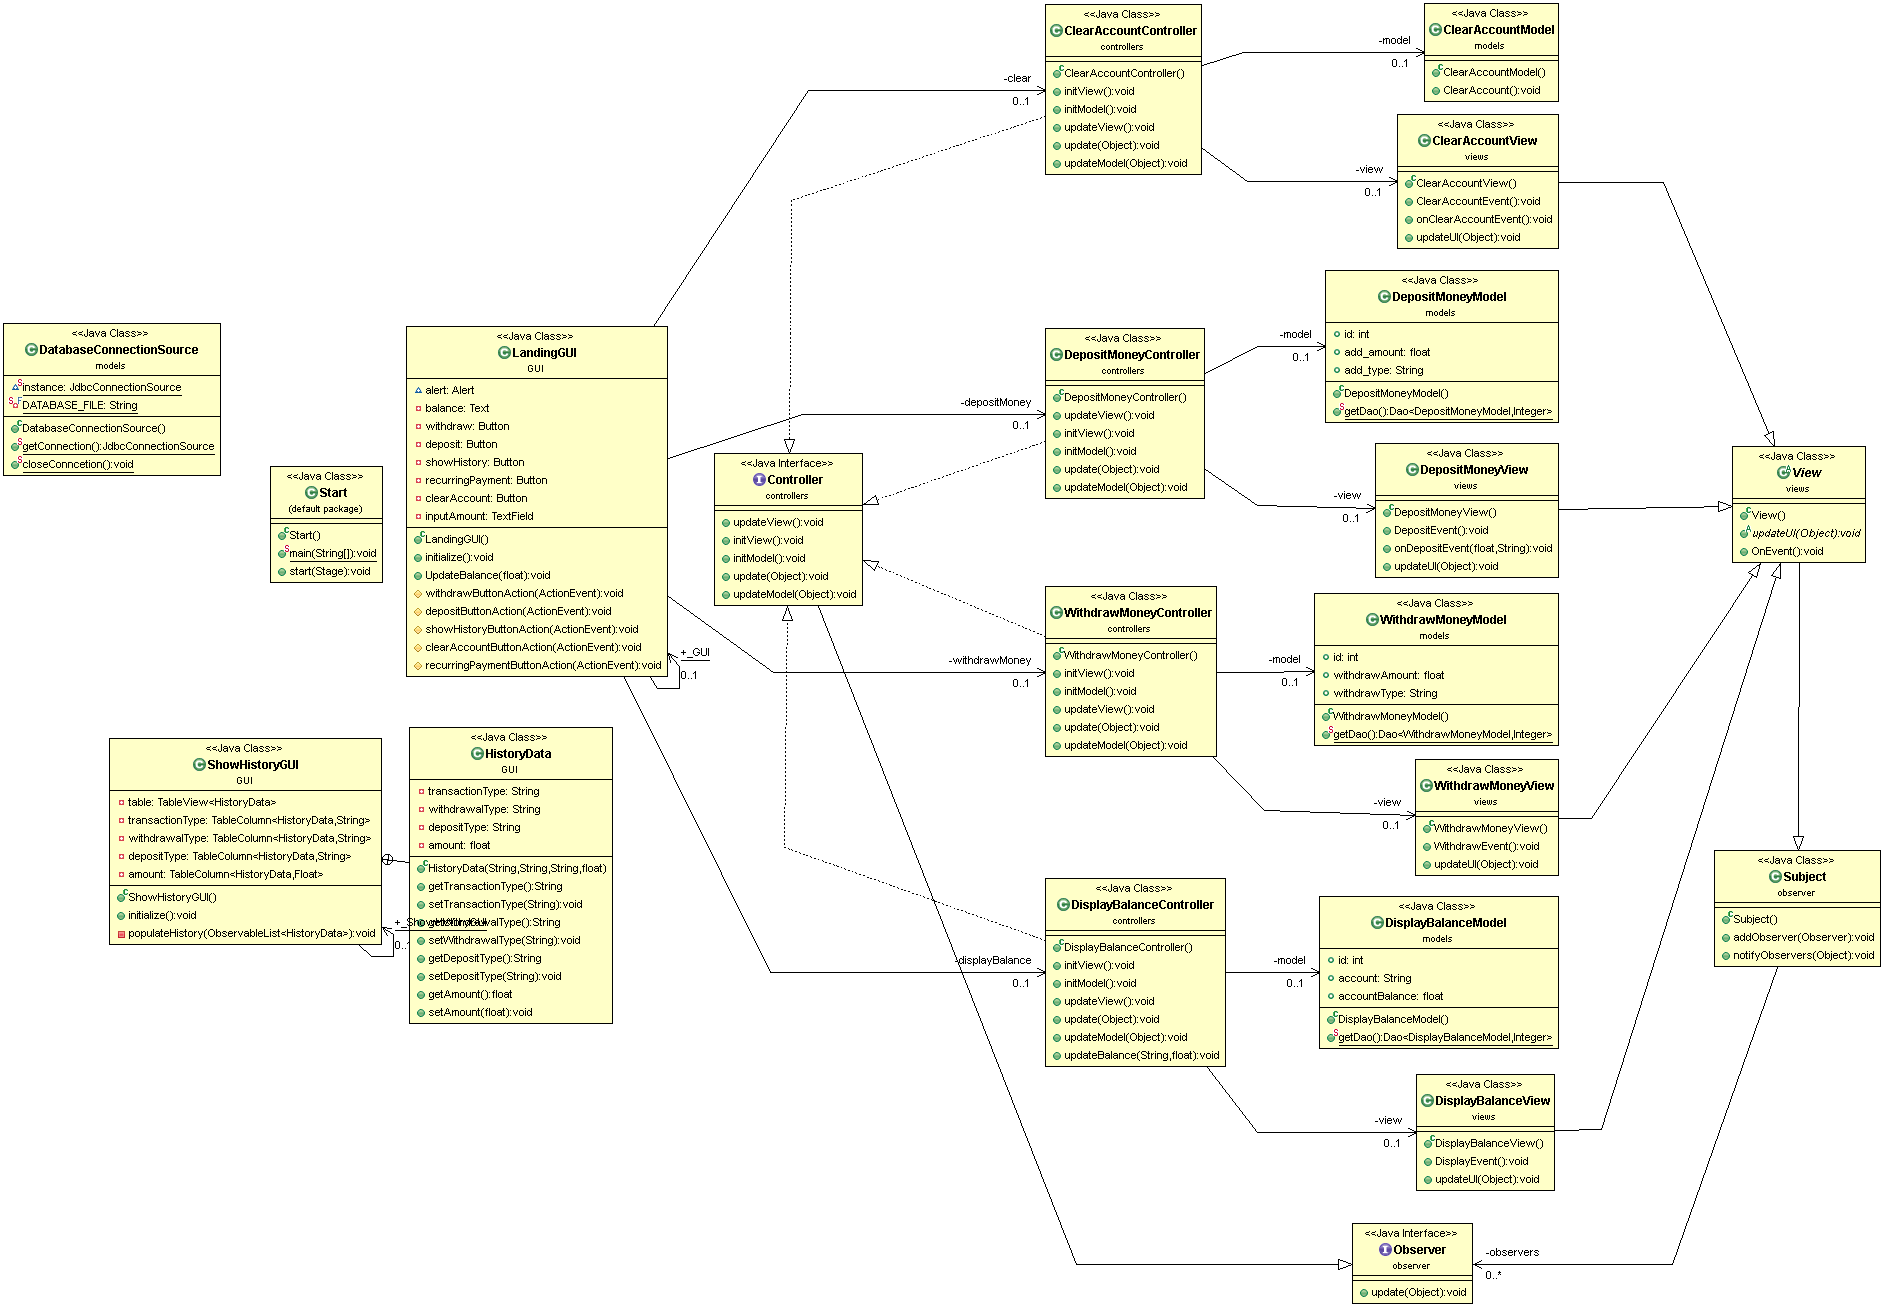
\includegraphics[width=110mm]{class_diagram.gif}
%  \caption{Withdraw Button}
%\end{figure}

\subsubsection{Deposit Button}

The deposit button of the basic options subsection when clicked on will increase the current balance by the number specified in “Enter Amount”

% Deposit button Image
%\begin{figure}[h!]
%  \centering
%  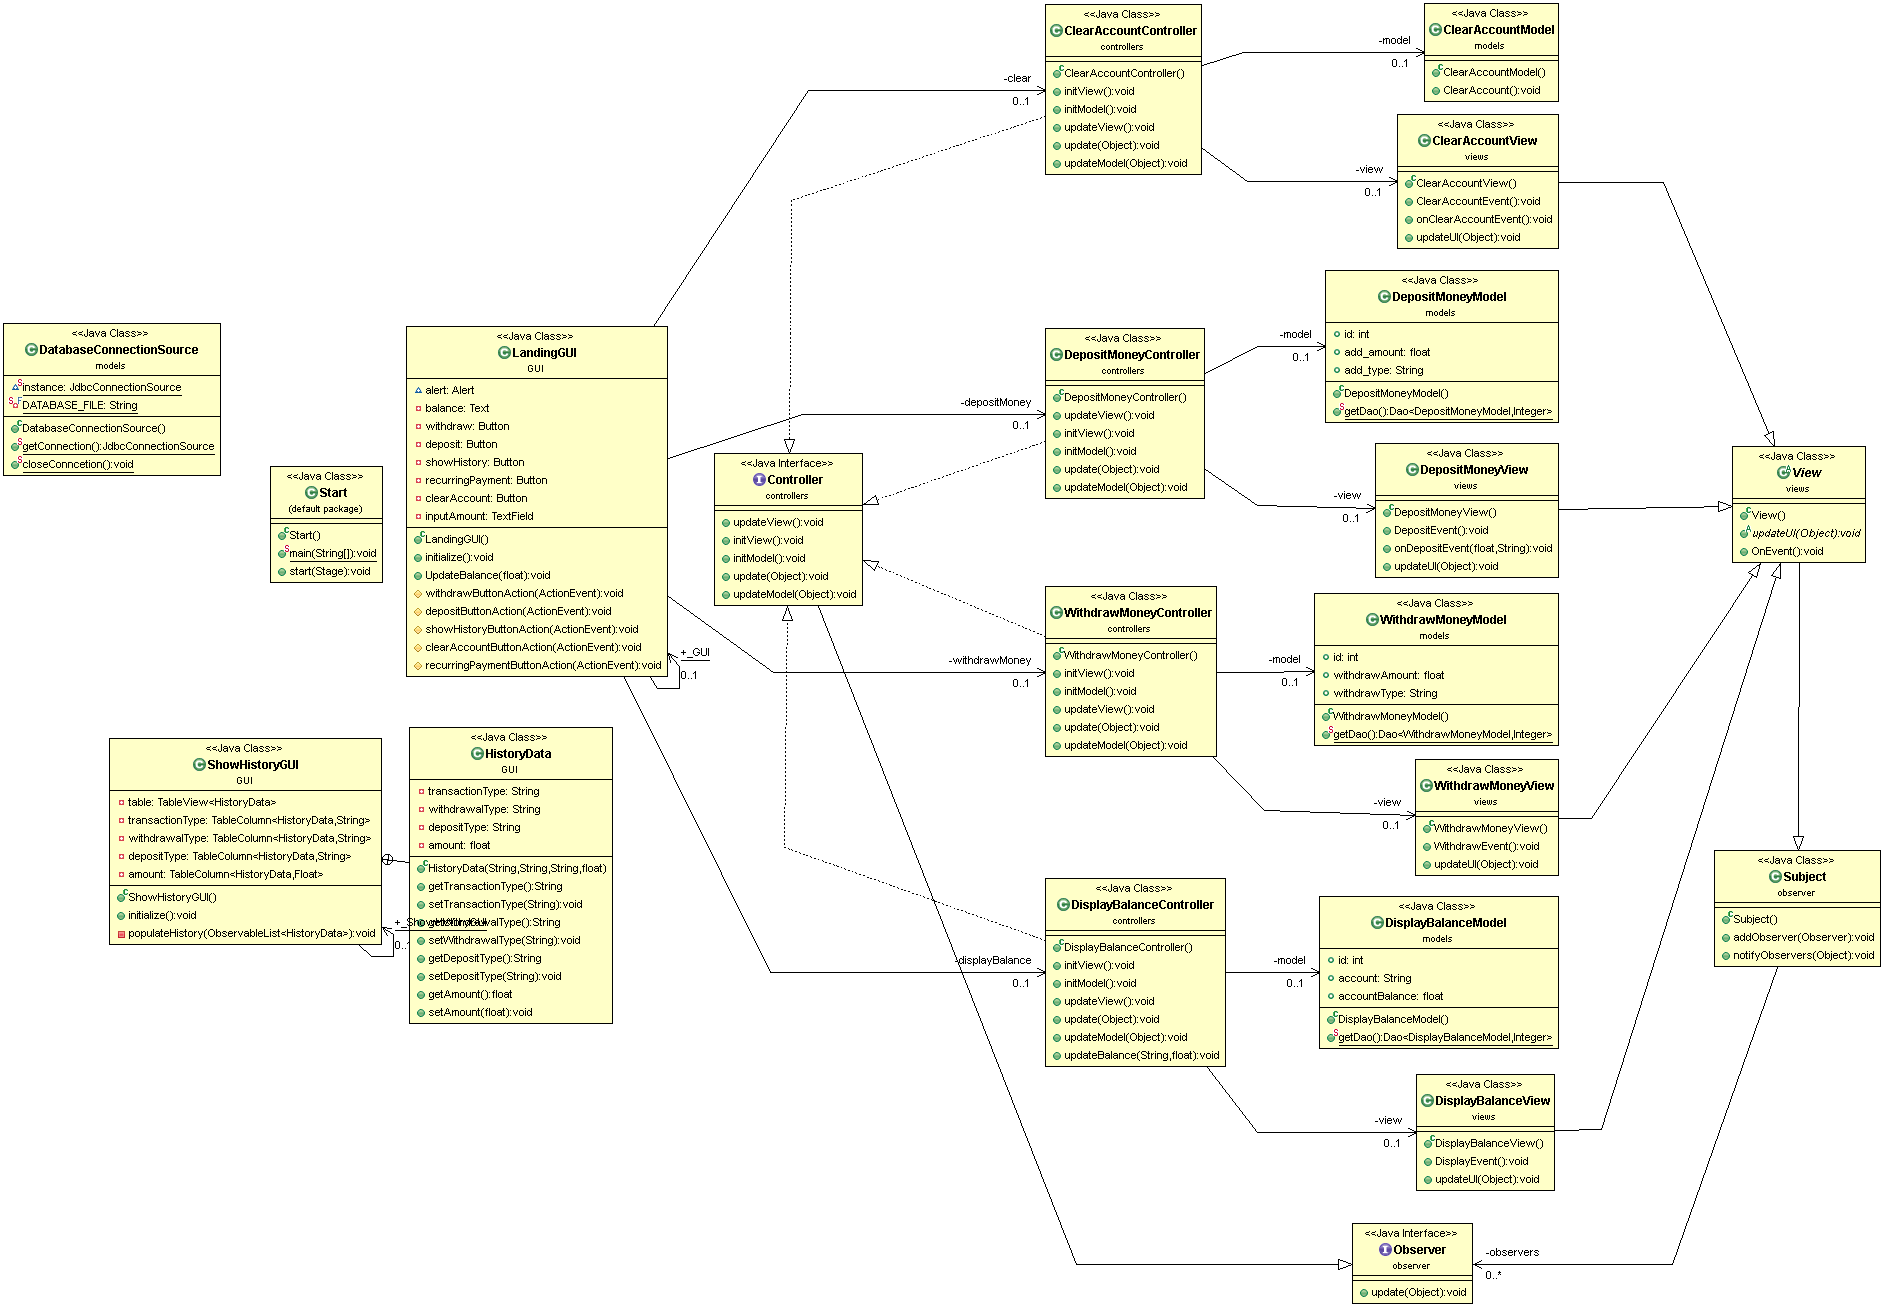
\includegraphics[width=110mm]{class_diagram.gif}
%  \caption{Deposit Button}
%\end{figure}

\subsubsection{Show History Button}
The show history button of the basic options subsection when clicked upon will show the past transactions that the user has done such as deductions and deposits.

% Show history button Image
%\begin{figure}[h!]
%  \centering
%  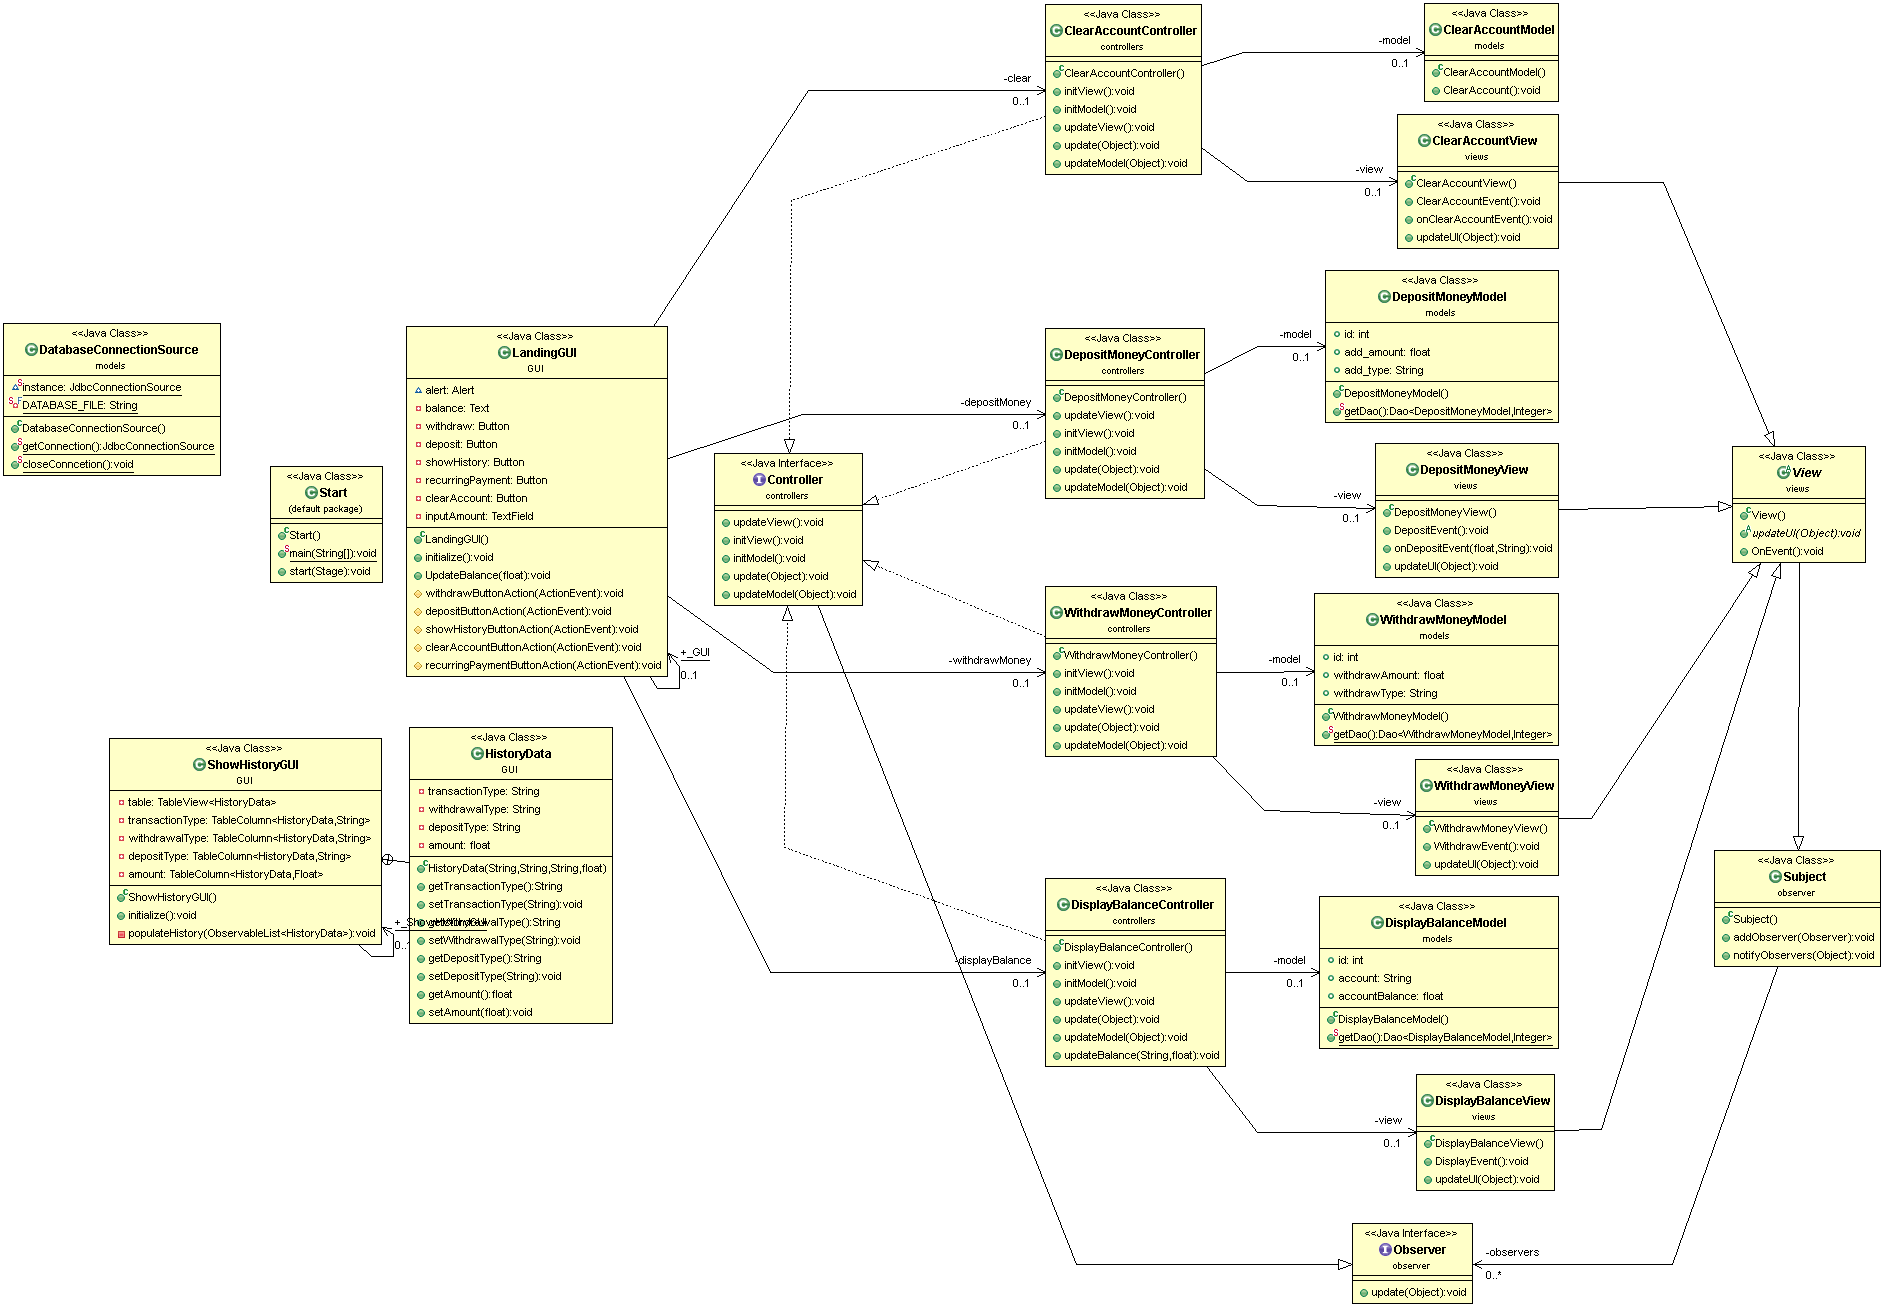
\includegraphics[width=110mm]{class_diagram.gif}
%  \caption{Show history Button}
%\end{figure}

\subsubsection{Setup Recurring Payment Button}
The setup recurring payment button of the advanced options subsection will set up a system where a certain amount will be automatically deducted or incremented from current balance for a specific time interval, such as the first of every month, or every week.

% Show history button Image
%\begin{figure}[h!]
%  \centering
%  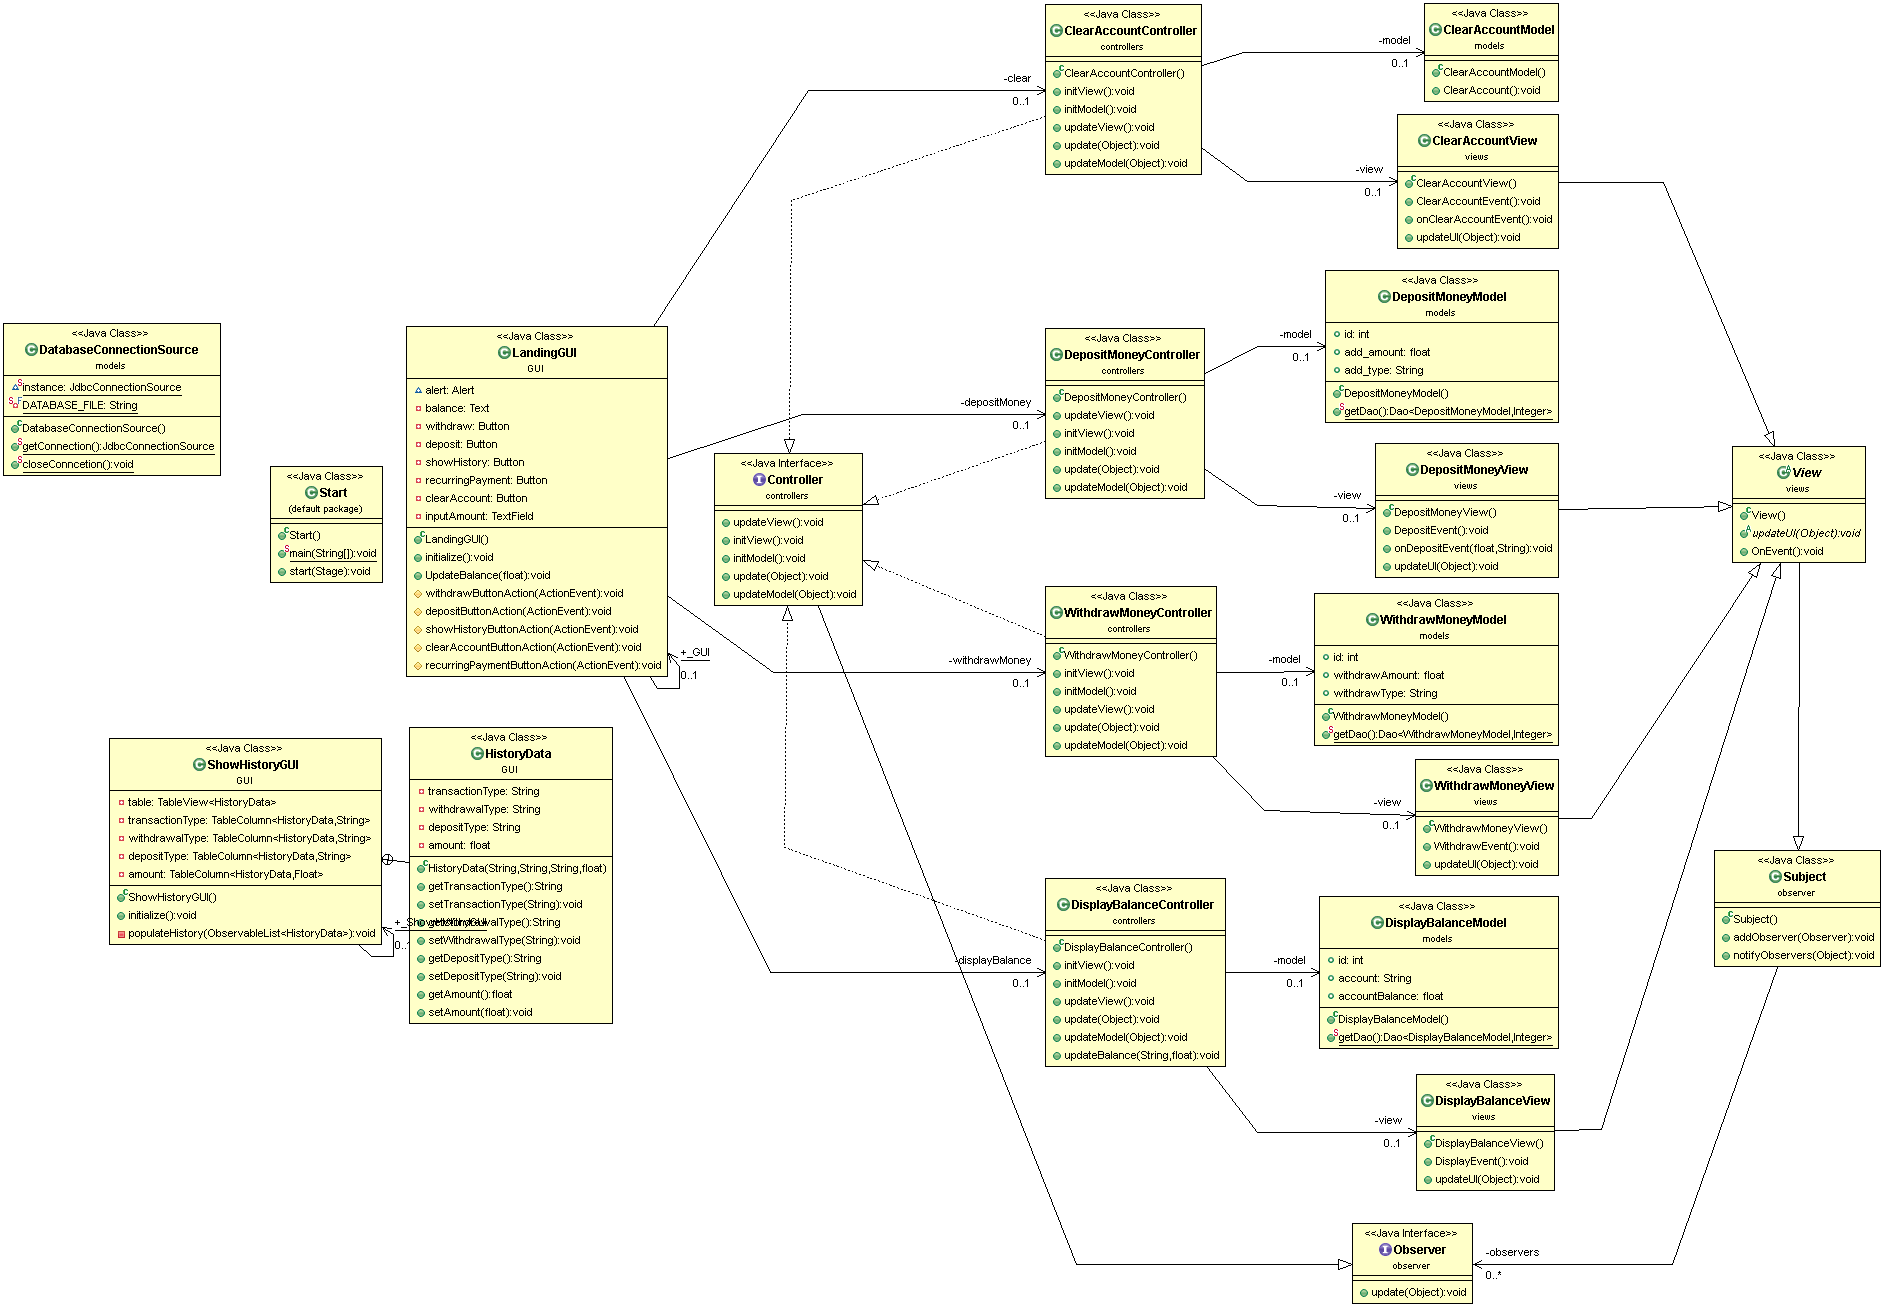
\includegraphics[width=110mm]{class_diagram.gif}
%  \caption{Show history Button}
%\end{figure}

\subsubsection{Clear Account Button}
The clear account button of the advanced options subsection will delete the current account and reset the application back to the clear default state.

% Clear Account button Image
%\begin{figure}[h!]
%  \centering
%  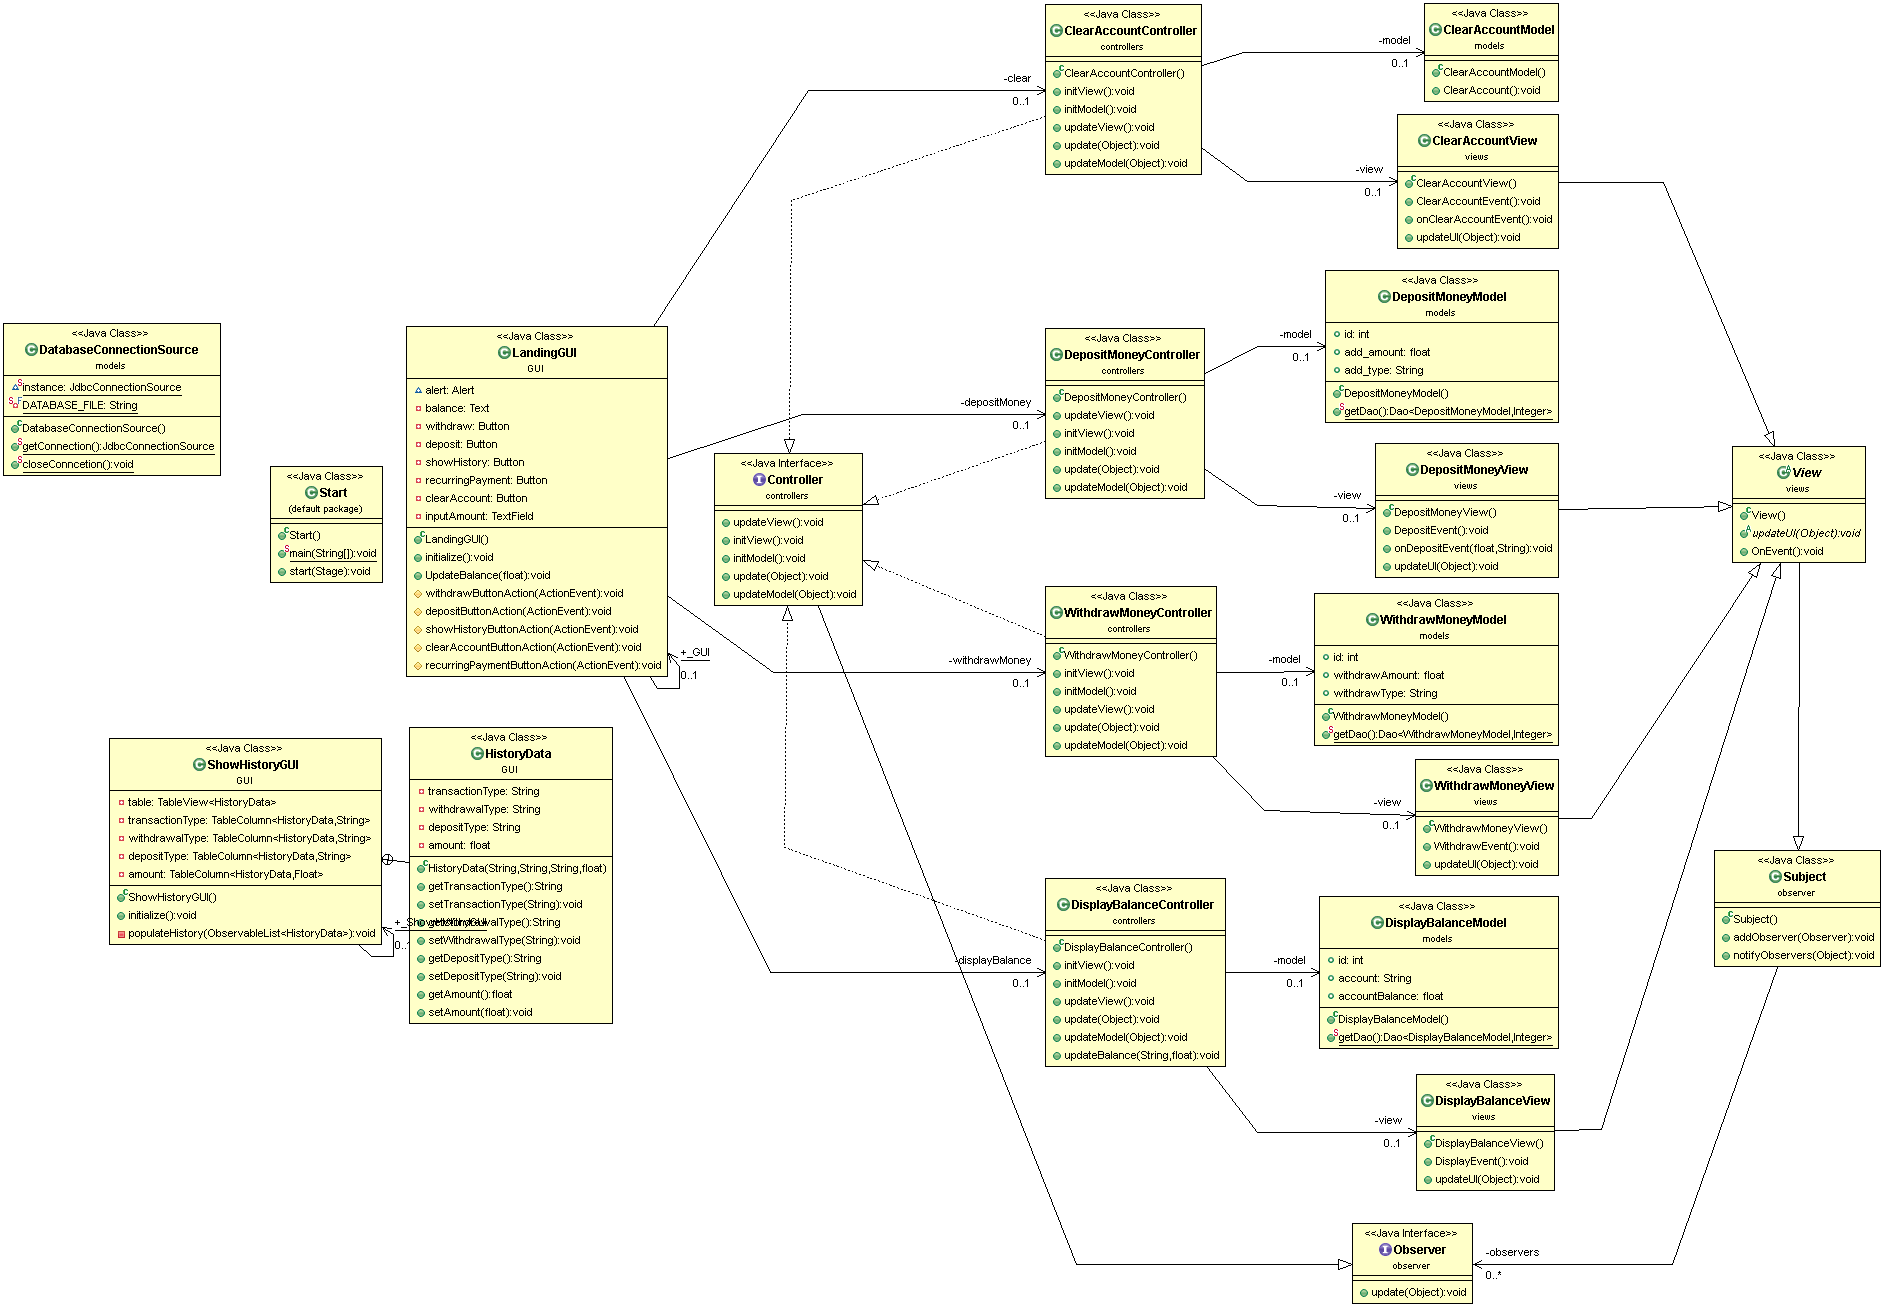
\includegraphics[width=110mm]{class_diagram.gif}
%  \caption{Clear Account Button}
%\end{figure}

\subsubsection{Enter Amount Field}
The enter amount field located in the center of the GUI is where the amount is typed to perform operations on the current balance such as typing in a certain amount and the clicking on withdraw to deduct that amount from the current balance.

% Enter Amount Image
%\begin{figure}[h!]
%  \centering
%  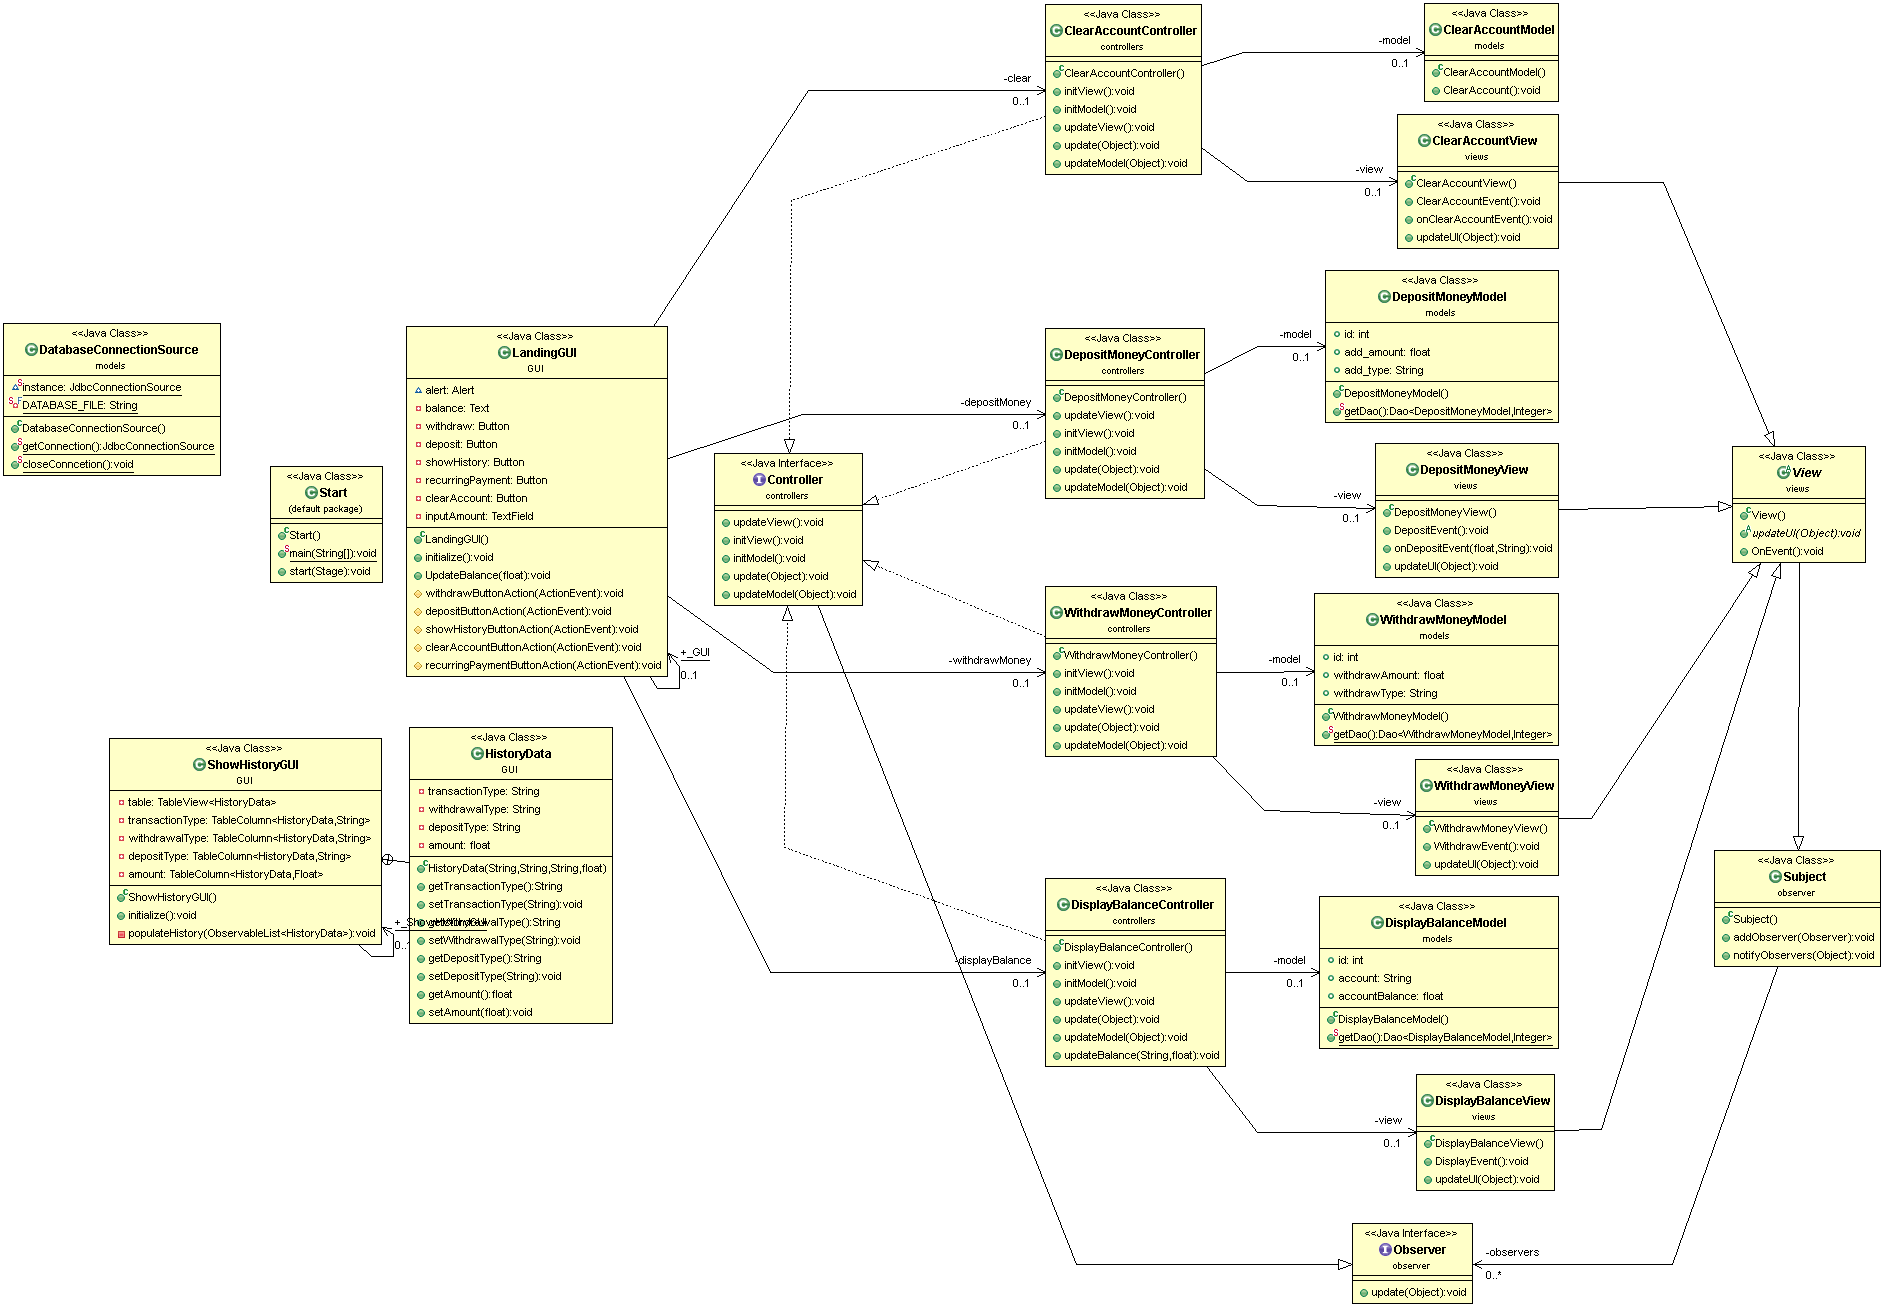
\includegraphics[width=110mm]{class_diagram.gif}
%  \caption{Enter Amount Field}
%\end{figure}

\subsubsection{Current Balance Field}
The current balance field at the bottom of the GUI is where the users current balance is displayed the amount of money that the user currently has to alter.

% Current Balance Field Image
%\begin{figure}[h!]
%  \centering
%  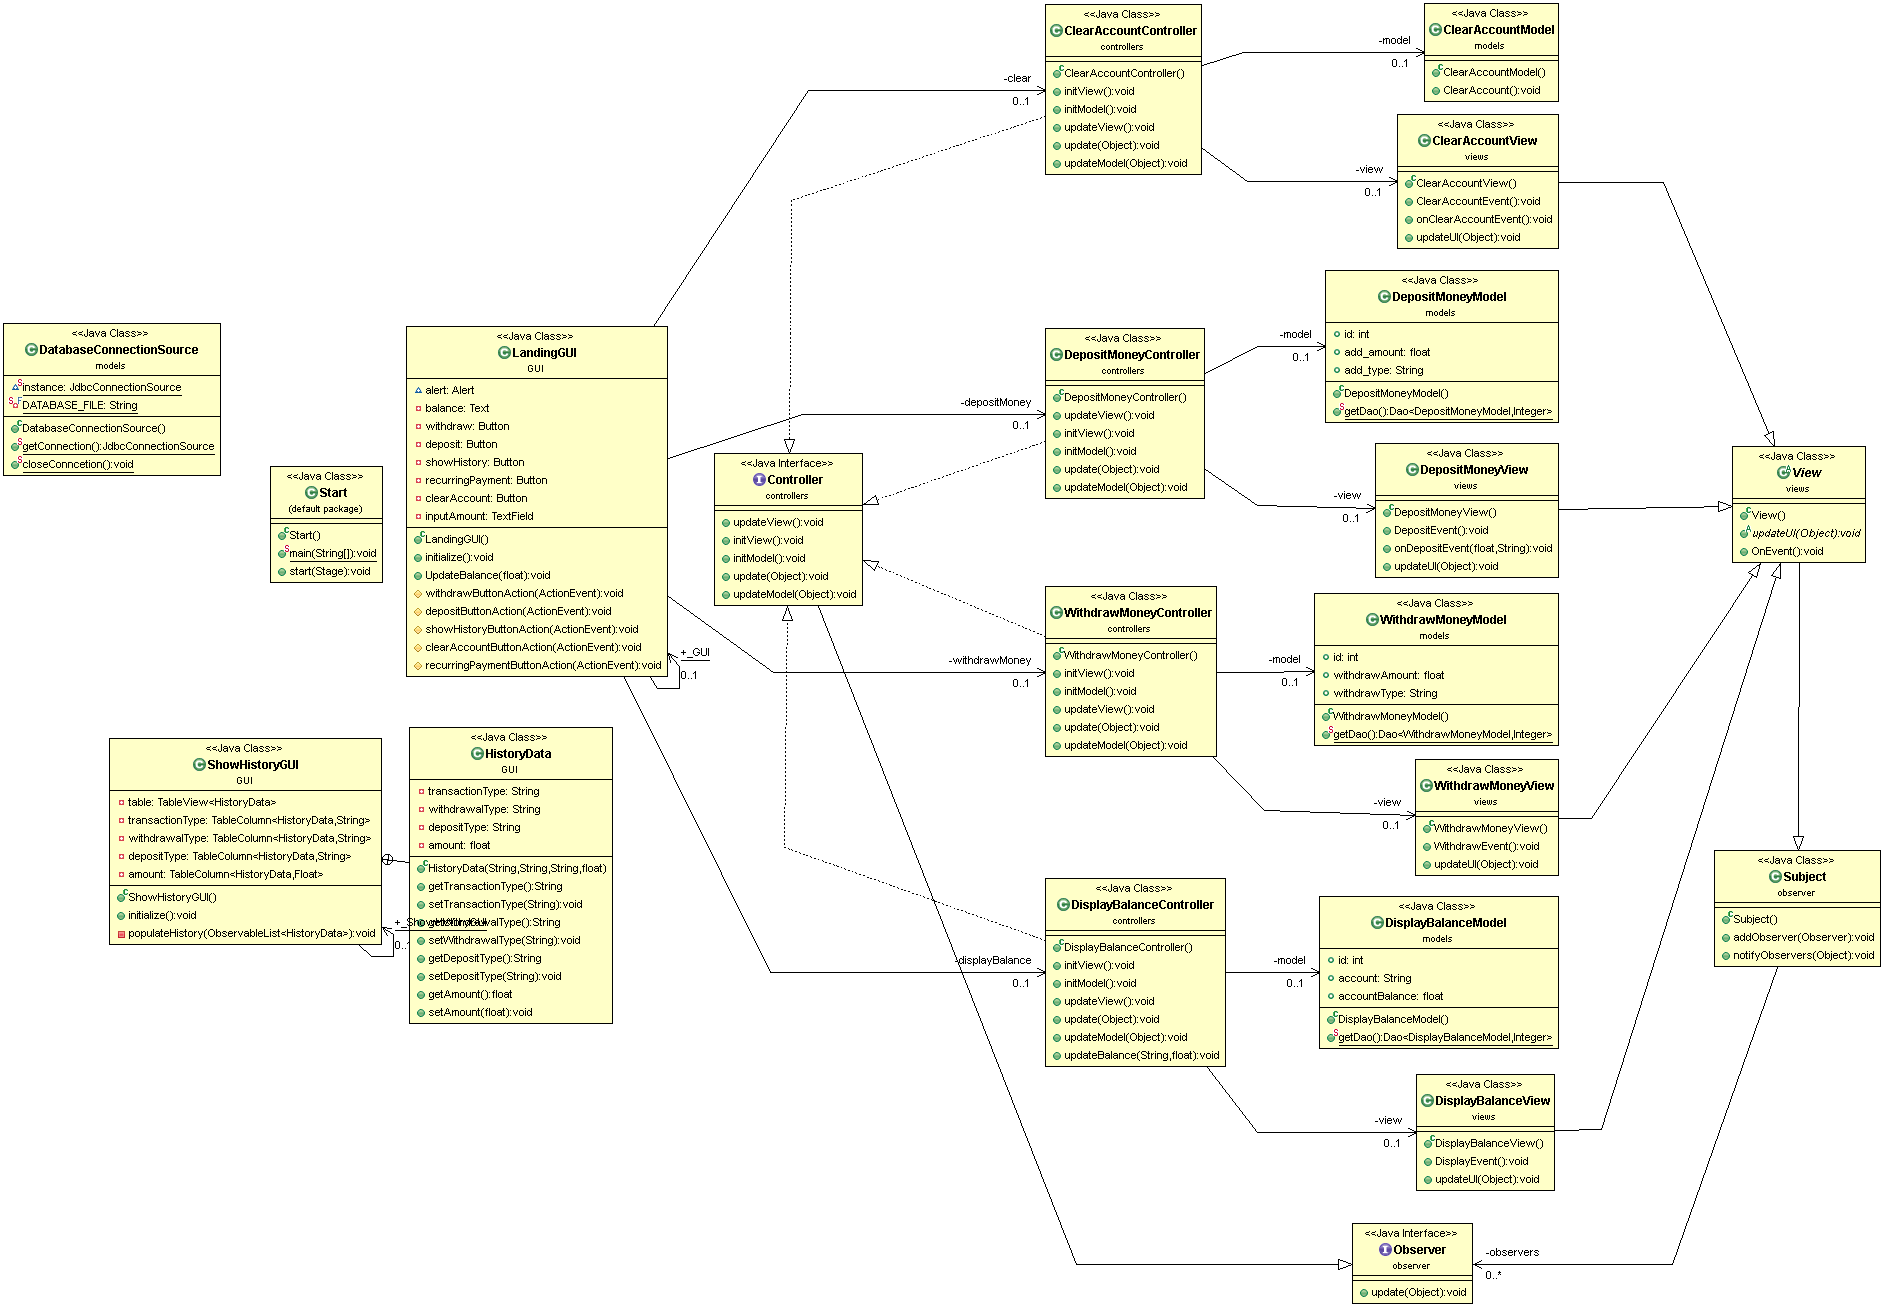
\includegraphics[width=110mm]{class_diagram.gif}
%  \caption{Current Balance Field}
%\end{figure}


\section{Dynamic Design Scenarios}
As explained, our software offers many functionalities that allows the user to interact with it. These functionalities were developed based on the gathered user stories. It includes: Deposit Amount, Withdraw Amount, Show Balance, Show History, Clear History, and Display GUI. 

\subsection{Deposit Amount}
Our software gives the user basic functionality such as “Deposit Amount”, which allows them to simply enter an amount to be saved into the “Deposit” section of the account. Once stored, the data can be used by other functionalities to extend the user interactability with the system. 

\subsubsection{Deposit Amount - Sequence Diagram}
% Doenst support static gif. we'll need to convert to another format
%\begin{figure}[h!]
%  \centering
%  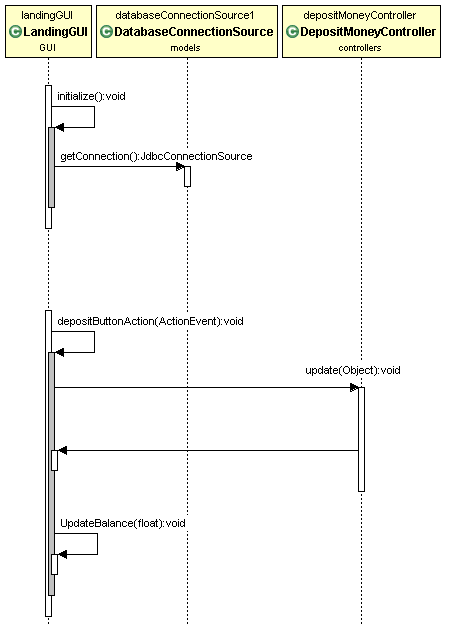
\includegraphics[width=110mm]{deposit_sequence.gif}
%  \caption{Deposit Sequence Diagram}
%\end{figure}


The Deposit Amount use case is a basic functionality that is invoked from the GUI. When the GUI is launched, it establishes a connection with the database and then waits for user inputs. Once the user entered an amount into the Deposit’s input box and confirmed their action by pressing the “Deposit Amount” button, the function depositButtonAction(ActionEvent) is called which tells the DepositMoneyController to update the Model. When updated, the DepositMoneyController will signal the GUI that the information has been successfully updated and that it needs to display the new information. The GUI will then call UpdateBalance(float) which will finally update the displayed balance to reflect the new amount.


\subsection{Withdraw Amount}
Similar to the “Deposit Amount” use case, “Withdraw Amount” is another basic functionality that allows the user to interact with the system. It requires the user to input a withdrawal amount which is saved into the “Withdraw” section of the account. 

\subsubsection{Withdraw Amount - Sequence Diagram}
% Doenst support static gif. we'll need to convert to another format
%\begin{figure}[h!]
%  \centering
%  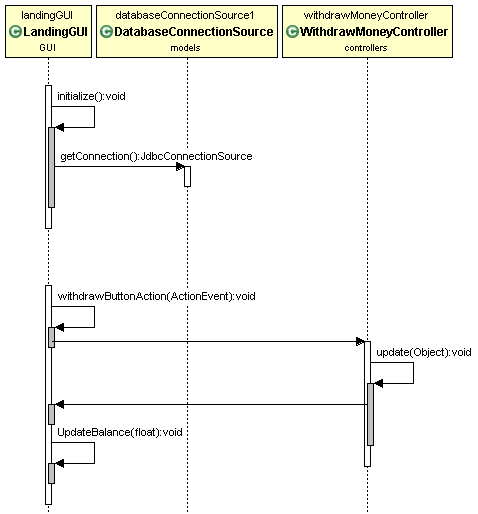
\includegraphics[width=110mm]{withdraw_sequence.gif}
%  \caption{Withdraw Sequence Diagram}
%\end{figure}

This use case functions very similarly to the “Deposit Amount” use case. It establishes a database connection when the GUI is launched and waits for user inputs. Once a withdrawal amount has been entered and confirmed by the user, it triggers the withdrawButton(ActionEvent) function which informs the WithdrwaMoneyController to update the Model. The controller will then update the model and inform the GUI that the changes has been successfully applied. The GUI will then call UpdateBalance(float) function which will update the displayed balance to reflect the new amount.

\subsection{Show Balance} 
“Show Balance” is a feature that allows the user to see the difference between their monthly earning and spending. This amount can be negative or positive to reflect the user’s monthly money situation (Negative amount: User spends more than they earn, Positive amount: the opposite). This use case solidifies the intent of our software which allows the user to know about their spending habits for a given period of time.

Additionally, the balance amount is shown on the main window of the software and is constantly updated when specific actions are made. For instance, a successful Deposit or Withdraw amount input would update the balance once the action is complete. 


\subsection{Show History} 
“Show History” is a functionality that allows the user to see all previous Deposit and Withdraw inputs to review certain purchases they have made or certain deposits they have forgotten for instance.. When the “Show History” button is pressed, a new window containing the information will pop up on top of the main window. This new window is independent to the main window and can be freely manipulated by the user. 

Within this new window, it will display a table with all Deposit and Withdraw inputs since the beginning. The data is sorted by the input date from newest to oldest. The user can resume their normal activity with the software regardless of whether the “Show History” window is active or not. Although, if the user inputs more data with the history window still open, it will not display the new additions and would require the user to reopen the same window to see the changes.


\subsection{Clear History}
“Clear History” is another functionality that allows the user to remove all data that has ever been saved into the software. This allows any old or unnecessary information to be removed allowing the user to only see recent information. By pressing the “Clear History” button, it will empty all tables within the database such as Deposit and Withdraw amounts.

\subsection{Display GUI}
“Display GUI” is a feature that allows the user to easily interact with the system.The GUI simplifies the number of steps required for the user to carry out an action on the software by allowing them to simply type into input boxes and press on buttons to confirm their actions.This feature also compacts all other features and functionalities into one window which greatly improves the user’s experience. 

\subsubsection{MVC Sequence Diagram}

The system was developed around the MVC model with heavy use of the Observer Pattern. With the implementation of the GUI, we have made significant changes to the structure of this model by making the GUI a view component. Other than these changes, our system behaves exactly how MVC works. 

In the previous “Deposit Amount” and “Withdraw Amount” use cases described above, the respective sequence diagrams only explained the surface on how those functionalities work relative to all subsystems and units.

The sequence diagram below shows in more detail how MVC with the Observer Pattern functions in our system.    

% Doenst support static gif. we'll need to convert to another format
%\begin{figure}[h!]
%  \centering
%  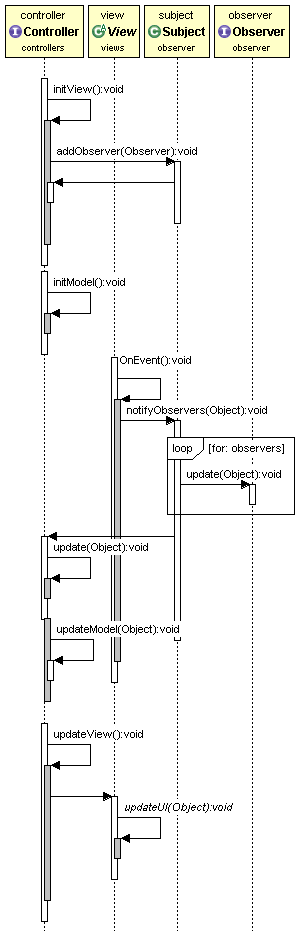
\includegraphics[width=110mm]{mvc_sequence.gif}
%  \caption{MVC Sequence Diagram}
%\end{figure}


\end{document}